%%%%%%%%%%%%%%%%%%%%%%%%%%%%%%%%%%%%%%%%%
% University Assignment Title Page 
% LaTeX Template
% Version 1.0 (27/12/12)
%
% This template has been downloaded from:
% http://www.LaTeXTemplates.com
%
% Original author:
% WikiBooks (http://en.wikibooks.org/wiki/LaTeX/Title_Creation)
%
% License:
% CC BY-NC-SA 3.0 (http://creativecommons.org/licenses/by-nc-sa/3.0/)
% 
% Modified for COSC480/490 by: Louis Whitburn
% Lech Szymanski (8/3/18)

\documentclass[12pt]{article}
\usepackage[draft]{cosc4x0style}

\usepackage{listings}

\usepackage{biblatex}

\usepackage{xcolor}

% Encoding goodness that I usually expect to rely on...
\usepackage[T1]{fontenc}
\usepackage[utf8]{inputenc}

\definecolor{codegreen}{rgb}{0,0.6,0}
\definecolor{codegray}{rgb}{0.5,0.5,0.5}
\definecolor{codepurple}{rgb}{0.58,0,0.82}
\definecolor{backcolour}{rgb}{0.95,0.95,0.92}

\lstset{
	backgroundcolor=\color{backcolour},   
	commentstyle=\color{codegreen},
	keywordstyle=\color{blue},
	numberstyle=\color{codegray},
	stringstyle=\color{codepurple},
	breaklines=true,
	breakatwhitespace=true,
	numbers=left,
	basicstyle=\ttfamily
}
 
\usepackage{amssymb}
\usepackage{amsmath}

\usepackage{graphicx}

\usepackage{wrapfig}

\addbibresource{bibliography.bib}

% The sorts of macros that I (Dave) normally use when working with LaTeX
\newcommand{\note}[2][red]{\textcolor{#1}{#2}}
\newcommand{\notedme}[1]{\note[blue]{[<Dave> #1]}}
\newenvironment{scaffold}{\color{red}}{}
\newcommand{\change}[2][]{\textcolor{orange}{#2}}

% To compile the final version of the report (which will remove all the todo content)
%\usepackage{cosc4x0style}

% Specify project code 480 or 490
\papercode{490}

% Your project title
\title{Kalman Filtering in Verilog}

% Your name
\author{Louis \textsc{Whitburn}}
\studentid{2548261}

% Names of your supervisors, separated by line break '\\'
\supervisors{
  Dr.\@ Tim \textsc{Molteno} \\
  Dr.\@ David \textsc{Eyers}
}

% Date, change the \today to a set date if you want to be precise
\reportdate{\today}

\begin{document}


\maketitle

\begin{abstract}

With the surge in growth of the UAV and smartphone industry, there continues to be significant demand for accurate and low power methods to measure and estimate orientation. The simplest method of estimating a device's orientation is by comparing the device's orientation to gravity, i.e.\@ by using accelerometers. This method is very easy to implement, however becomes very inaccurate when the device is actually accelerating. The solution to this is to combine multiple sensors (via a process called sensor fusion), such as gyroscope measurements and magnetometer data. One of the most well known methods of achieving this\notedme{too many `this's---you've used one in each of the preceding three sentences. Sometimes, it will be clearer to repeat an explicit noun. There's also the risk of ambiguity as to what `this' is referring to in each instance.} is through the Kalman filter, however this requires some fairly computationally expensive matrix mathematics, which limits potential performance, and results in greater than necessary power drain. My project explores the implementation of this in hardware, and the tradeoffs between hardware resource consumption and performance. In particular, hardware has significant flexibility in representation of numerical quantities, and choices of representation affect the accuracy of the inferred orientation.
\notedme{Good, but you don't seem to be answering Brendan's question from the talks---and he could well be one of the academics reading this report.}

\section{Introduction}

The sales of cell phones may have slowed down in recent years, but still exceeds one billion units sold per year \cite{Mongardini_2020}. The smartphone market is only one example of an area that requires accurate orientation data to operate correctly, e.g.\@ for augmented reality applications. State estimation using the Kalman filter is still considered the ``go-to'' approach to solving this problem, however many solutions continue to do this mostly in software \cite{ayub_2012}. This isn't ideal from an efficiency standpoint, since software, while being very flexible, is not particular power efficient or fast. Several hardware-based approaches have been developed, however they are either too complex \cite{mills_2016} to be synthesized to a cheap FPGA, or are encumbered with intellectual property restrictions. I aim to produce a design that can be synthesised to any FPGA (of a certain size)\notedme{If there's a size restriction, it's not clear that this is really `any' anymore?} and interfaced with sensors to give an estimate of orientation.

The primary motivation behind this is reduced power consumption, although there will be an increase in performance as well. Given that most software Kalman filter implementations are already ``good enough'', i.e.\@ the reported data is reasonably accurate, then this increase in performance would likely simply be a justification to lower the data input frequency to further lower power consumption. This\notedme{what `this'?} would also increase flexibility, allowing the CPU cycles that were used running the Kalman filter in software to do more useful work.
\notedme{This does essentially answer Brendan's question (although I'd suggest still doing so in the abstract, too), however I think you could be even more direct. Existing approaches are good enough (i.e., for their target application domains, although you don't explicitly say this), but also, there's the potential to do better. If it's clear that that's the case, that's more than enough justification for the project in my mind---noting that it's also fine just to look into the project because you find the topics interesting...}

\section{Background}

Before moving on \notedme{Unnecessary text to the left?}, I would like to introduce the Kalman filter and Hardware Description languages. I would also like to comment on the typical differences between software and hardware solutions to problems.
\notedme{Say why you're doing so, not necessarily just \emph{that} you're doing so?}

\subsection{Inertial Measurement Units}

An inertial measurement unit is a device which reports the acceleration, and angular velocity of an object, typically by using accelerometers and gyroscopes. When combined with post-processing they can also report on the device's orientation. One method for integrating multiple sources and updating the understanding of the system is through sequential inference.

\subsection{Sequential Inference}

Sequential inference \cite{morrison_2016} is the process of repeatedly adding information to a model of a system to improve our understanding of the state that system is in. In particular, we can derive \cite{morrison_2016}

\begin{equation}
	\label{si}
	P(S | D_1, m) = {P(D_1 | S, m) P(S | m) \over P(D_1 | m)}
\end{equation}

\noindent Where $S$ is the state, $D_n$ are the measurements at time step $n$, and $m$ is the model. What this equation is saying is that probability of the system being in some state, given some measurements and a model, is the product of the probability of making some measurement, given the state and the model weighted by the ratio between the probability of being in that state (given a model of the system) and the probability of making those measurements (given a model of the system). This is simply an application of Bayes' Theorem:

\begin{equation}
	P(A | B) = {P(B|A) P(A) \over P(B)}
\end{equation}

The significance of being based off of Bayes's Theorem is that it means that equation \ref{si} can be composed to give

\begin{equation}
	P(S|D_2,D_1,m) = {P(D_2|D_1,S,m) \over P(D_2|D_1,m)} P(S | D_1, m)
\end{equation}

\noindent Thus we can add more measurements to our system to gain a better understanding of the state that it is in. One of the most widely used applications of sequential inference is via the Kalman filter.

\subsubsection{Kalman Filter}

The Kalman filter \cite{kalman_1960} is the ``go to'' algorithm \notedme{Not sure `go to' is formal or precise enough? Maybe it is...} for estimating the state (e.g.\@ orientation) of a system from multiple noisy sensors. It works by using a model of the system to predict the future state of that system, and then (after some time step), comparing that predicted state to the measured state.

The first two steps are to predict how the system will evolve:
\begin{eqnarray}
	\mathbf{\hat{x}}_{k | k-1} &=& \mathbf{F}_k \mathbf{\hat{x}}_{k-1|k-1} + \mathbf{B}_k \mathbf{u}_k \\
	\mathbf{P}_{k|k-1} &=& \mathbf{F}_k \mathbf{P}_{k-1 | k-1} \mathbf{F}^T_k + \mathbf{Q}_k
\end{eqnarray}

Here, $\mathbf{\hat{x}}_{k | k-1}$ and $\mathbf{P}_{k|k-1}$ are the \emph{a priori} (i.e.\@ without including any additional knowledge---the only knowledge we have are from the previous state---the $k-1|k-1$ subscripts) estimates of the state, and the covariance of the state. $\mathbf{F}_k$ is the state transition matrix, i.e.\@ it determines how the state changes through time. $\mathbf{B}_k$ is the control-input matrix applied to the control vector $\mathbf{u}_k$---these model any external input to the system, i.e.\@ if it was forced in a direction. Finally, $\mathbf{Q}_k$ is the covariance of the process noise, i.e.\@ the error / uncertainty that arises from the model. This uncertainty mainly arises from approximations made in the model (e.g.\@ linearisation), and from integration error (e.g.\@ if the measurement is velocity, then the estimate of position will drift if not corrected).

The next step is the update step. It first consists of the innovation stage---determining the difference between the predicted / forecast state and the observed state
\begin{eqnarray}
	\mathbf{\tilde{y}}_k &=& \mathbf{z}_k - \mathbf{H}_k \mathbf{\hat{x}}_{k|k-1} \\
	\mathbf{S}_k &=& \mathbf{H}_k \mathbf{P}_{k|k-1} \mathbf{H}^T_k + \mathbf{R}_k
\end{eqnarray}

\notedme{Just noting that AFAIK you don't need to use noindent if you \emph{are} actually starting a new paragraph---just explaining why I'm taking some of them out.}
Here $\mathbf{\tilde{y}}_k$ is that difference (residual), where $\mathbf{z}_k$ is the measured state and $\mathbf{\hat{x}}_{k|k-1}$ is the a priori estimate from before. $\mathbf{H}_k$ is the observation model, which maps the state space into the observation space---e.g.\@ when measuring depth via sonar the state space contains the depth, whereas the observation state contains the sonar round trip time. The observation model converts this (predicted) state into a (predicted) observation, in this case by dividing the distance by half the speed of sound in water. $\mathbf{S}_k$ is the residual of the covariance, where $\mathbf{R}_k$ is the covariance of the process noise, in the above example, this could arise from noisy sensors, and water currents and temperature differences slightly affecting the speed of sound in the water.

The second part of the update step is determining the Kalman gain:
\begin{eqnarray}
	\mathbf{K}_k = \mathbf{P}_{k|k-1} \mathbf{H}^T_k \mathbf{S}^{-1}_k
\end{eqnarray}

\noindent This generates a gain matrix which aims to minimise the \emph{a posteriori} (updated with the sensor observations)  residual, $\mathbf{\tilde{y}}_{k|k} = \mathbf{z}_k - \mathbf{H}_k \mathbf{\hat{x}}_{k|k}$.

The final part is generating these \emph{a posteriori} estimates
\begin{eqnarray}
	\mathbf{\hat{x}}_{k|k} &=& \mathbf{\hat{x}}_{k|k-1} + \mathbf{K}_k \mathbf{\tilde{y}}_k \\
	\mathbf{P}_{k|k} &=& (\mathbf{I} - \mathbf{K}_k \mathbf{H}_k)\mathbf{P}_{k|k-1}
\end{eqnarray}

\noindent where $\mathbf{\hat{x}}_{k|k}$ and $\mathbf{P}_{k|k}$ are the \emph{a posteriori} state estimate and state estimate covariance.
\notedme{(...but when continuing with a sentence, don't start with a capital letter, hence the change I made here.)}

Thus we have a mechanism to have our estimate of the state optimally track the actual state. In the above equations, the matrices (uppercase and bold) are of the size $n \times n$ and the vectors (lowercase and bold) are column vectors of the size $n \times 1$, where $n$ is the size of the estimated state. The observation space need not be the same size as the state space, thus if the size of the observation space is $m$, then $\mathbf{H}_k$ may be $m \times n$ and $\mathbf{z}_k$ may be $m \times 1$, however I will assume that $n = m$ for simplicity.

\subsection{Hardware Description Languages}

The 1975 MOS Technology 6502 consisted of approximately 3500 transistors. This is a comprehensible size, in that it is entirely possible to imagine it being designed by hand. On the other hand, the first CPU to introduce the x86 instruction set was the Intel 8086 back in 1978, made from some 29,000 transistors. An Intel Nehalem CPU from 12 years ago contains upwards of 750 million transistors. AMD's ``Epyc'' lineup of server CPUs contain up to 50 billion transistors per CPU. These would either be difficult and time consuming to design by hand (in the case of the 8086), or downright impossible to design by hand (the modern Nehalem and Epyc Rome CPUs). Thus the modern approach to chip design is based off using Hardware Description Languages (HDLs).

If I write a program in a language such as C, and target a conventional architecture, such as ARM or x86, then the code that I write is not the actual program---it only describes the program. For example, no CPUs contain a for loop instruction---a for loop in C is converted into (some variation of) a label, a comparison and a conditional jump to the position described by that label. The process of turning the description of the program to the actual program is ``compilation'', and this is fairly well understood. HDLs are the hardware equivalent of high level programming language---they do not describe logic gates and how they are connected, however they describe the behaviour of the hardware in a way such that it can be ``synthesized'' to the actual logic. For example, instead of having to describe each individual gate and connection in an adder, the designer can simply type \lstinline[language=Verilog]|a + b| and the synthesizer will generate the appropriately sized adder from that.

This can of course be used for more complex problems. For example, designing a (bad\footnote{Designing a ``good'' CPU is more complicated but entirely achievable---this one can even boot linux: \url{https://github.com/ultraembedded/biriscv}}) CPU in an HDL is almost trivial---all it needs is a suitably large array (to act as memory), some registers, and a few \lstinline[language=Verilog]|if| statements to determine what to do with each opcode.

Such a bad CPU\footnote{I want emphasize here just how bad this CPU is---inefficient, doesn't support a stack, no registers, no signed integers, no floating point numbers etc.\@---it is just a toy to show what can be done with HDLs such as Verilog} might be similar to the one included below:

\lstinputlisting[language=Verilog]{cpu-include.v}

Which gives the following output when simulated:

\lstinputlisting[numbers=none, backgroundcolor=\color{white}]{cpu-bench-result.txt}

In other words, it is a perfectly functioning CPU with it's own machine language code, which supports port-mapped IO (at a stretch), unconditional and conditional branching, and basic unsigned integer arithmetic.

\subsubsection{Icarus Verilog}

Icarus Verilog (Icarus) is an implementation of the Verilog HDL, available under the GNU General Public License (GPL). Icarus (or an alternative) is critical for testing hardware designs before trying them on hardware (e.g.\@ an FPGA) since it allows easy integration with a testbench, meaning the design can be simulated before synthesis to hardware. This is a critical part of the verification stage, as it allows bugs to be detected and fixed before hardware is manufactured.

\subsection{Hardware vs. Software Considerations}

Many of the matrix operations can be defined recursively, such as the matrix determinant of an $n \times n$ being a function of the determinants of the $(n-1) \times (n-1)$ minor matrices. If we consider imperative programming in a language such as C (again assuming that we are targeting a conventional architecture such as ARM or x86), then we try to avoid recursion as much as possible, favouring iterative approaches, since they tend to avoid some of the huge blow outs in runtime that can occur, since many recursive algorithms often calculate the same value multiple times. One example of this is the Fibonacci sequence:
\begin{eqnarray}
	F_0&&= 0 \\
	F_1&&= 1 \\
	F_n&&= F_{n-1} + F_{n-2}
\end{eqnarray}

\noindent Calculating $F_4$ requires knowing $F_3$ and $F_2$, but the calculation of $F_3$ also requires knowing $F_2$. A naive approach would result in several of the intermediate values being calculated multiple times, which is an inefficient use of time. One solution to this is memoisation, which is where the computed values would be cached to avoid re-computing them.

Hardware has similar concerns, except they manifest differently. Recursion in software takes up time, whereas recursion in hardware takes up space. This can be seen in \ref{recursion_space}, where it takes several pages to determine the determinant of a 4x4 matrix, but the calculation will be performed almost immediately. This should be considered in contrast to \ref{recursion_time}, which takes up a lot less space, and works for arbitrary sized matrices---however it will take much longer to execute (even if it were written in a lower level language).

These stem from the inherently sequential nature of software and the inherently parallel nature of hardware. It would be entirely possible to parallelise the matrix determinant code to use multiple processors / multiple cores, however this would introduce several challenges, thus the simple sequential program is the ``default'' (i.e.\@ most intuitively sensible option). If we now consider the hardware option, it would be possible for it to only have only one arithmetic unit, and rewrite the code such that only one mathematical operation is happening at any given time. However, this would introduce considerable complexity since we would need to store state (how far through the calculation we are), and the unit would need to be clocked---effectively turning it into a very specific CPU. Thus the parallel implementation can be considered the ``default'' for hardware.

\section{Progress}

\subsection{Python Kalman Filter}

The first phase of the project was getting a simple Kalman filter working. This was based on a simple one-dimensional cart moving backwards and forwards, with the measured quantity being position. In figure \ref{1d_position_fig} we can see the system handles both a fairly predictable motion as well as an unpredictable motion quite well. This is to be expected since we are measuring position, thus we expect the estimate of position to be fairly accurate (for obvious reasons). The estimate of velocity slowly converges to the actual velocity, however it has to re-converge after the bump. This is also expected since the bump was modelled as an impulse, which isn't a 100\% realistic scenario.

\begin{figure}[thp]
	\centering
	
	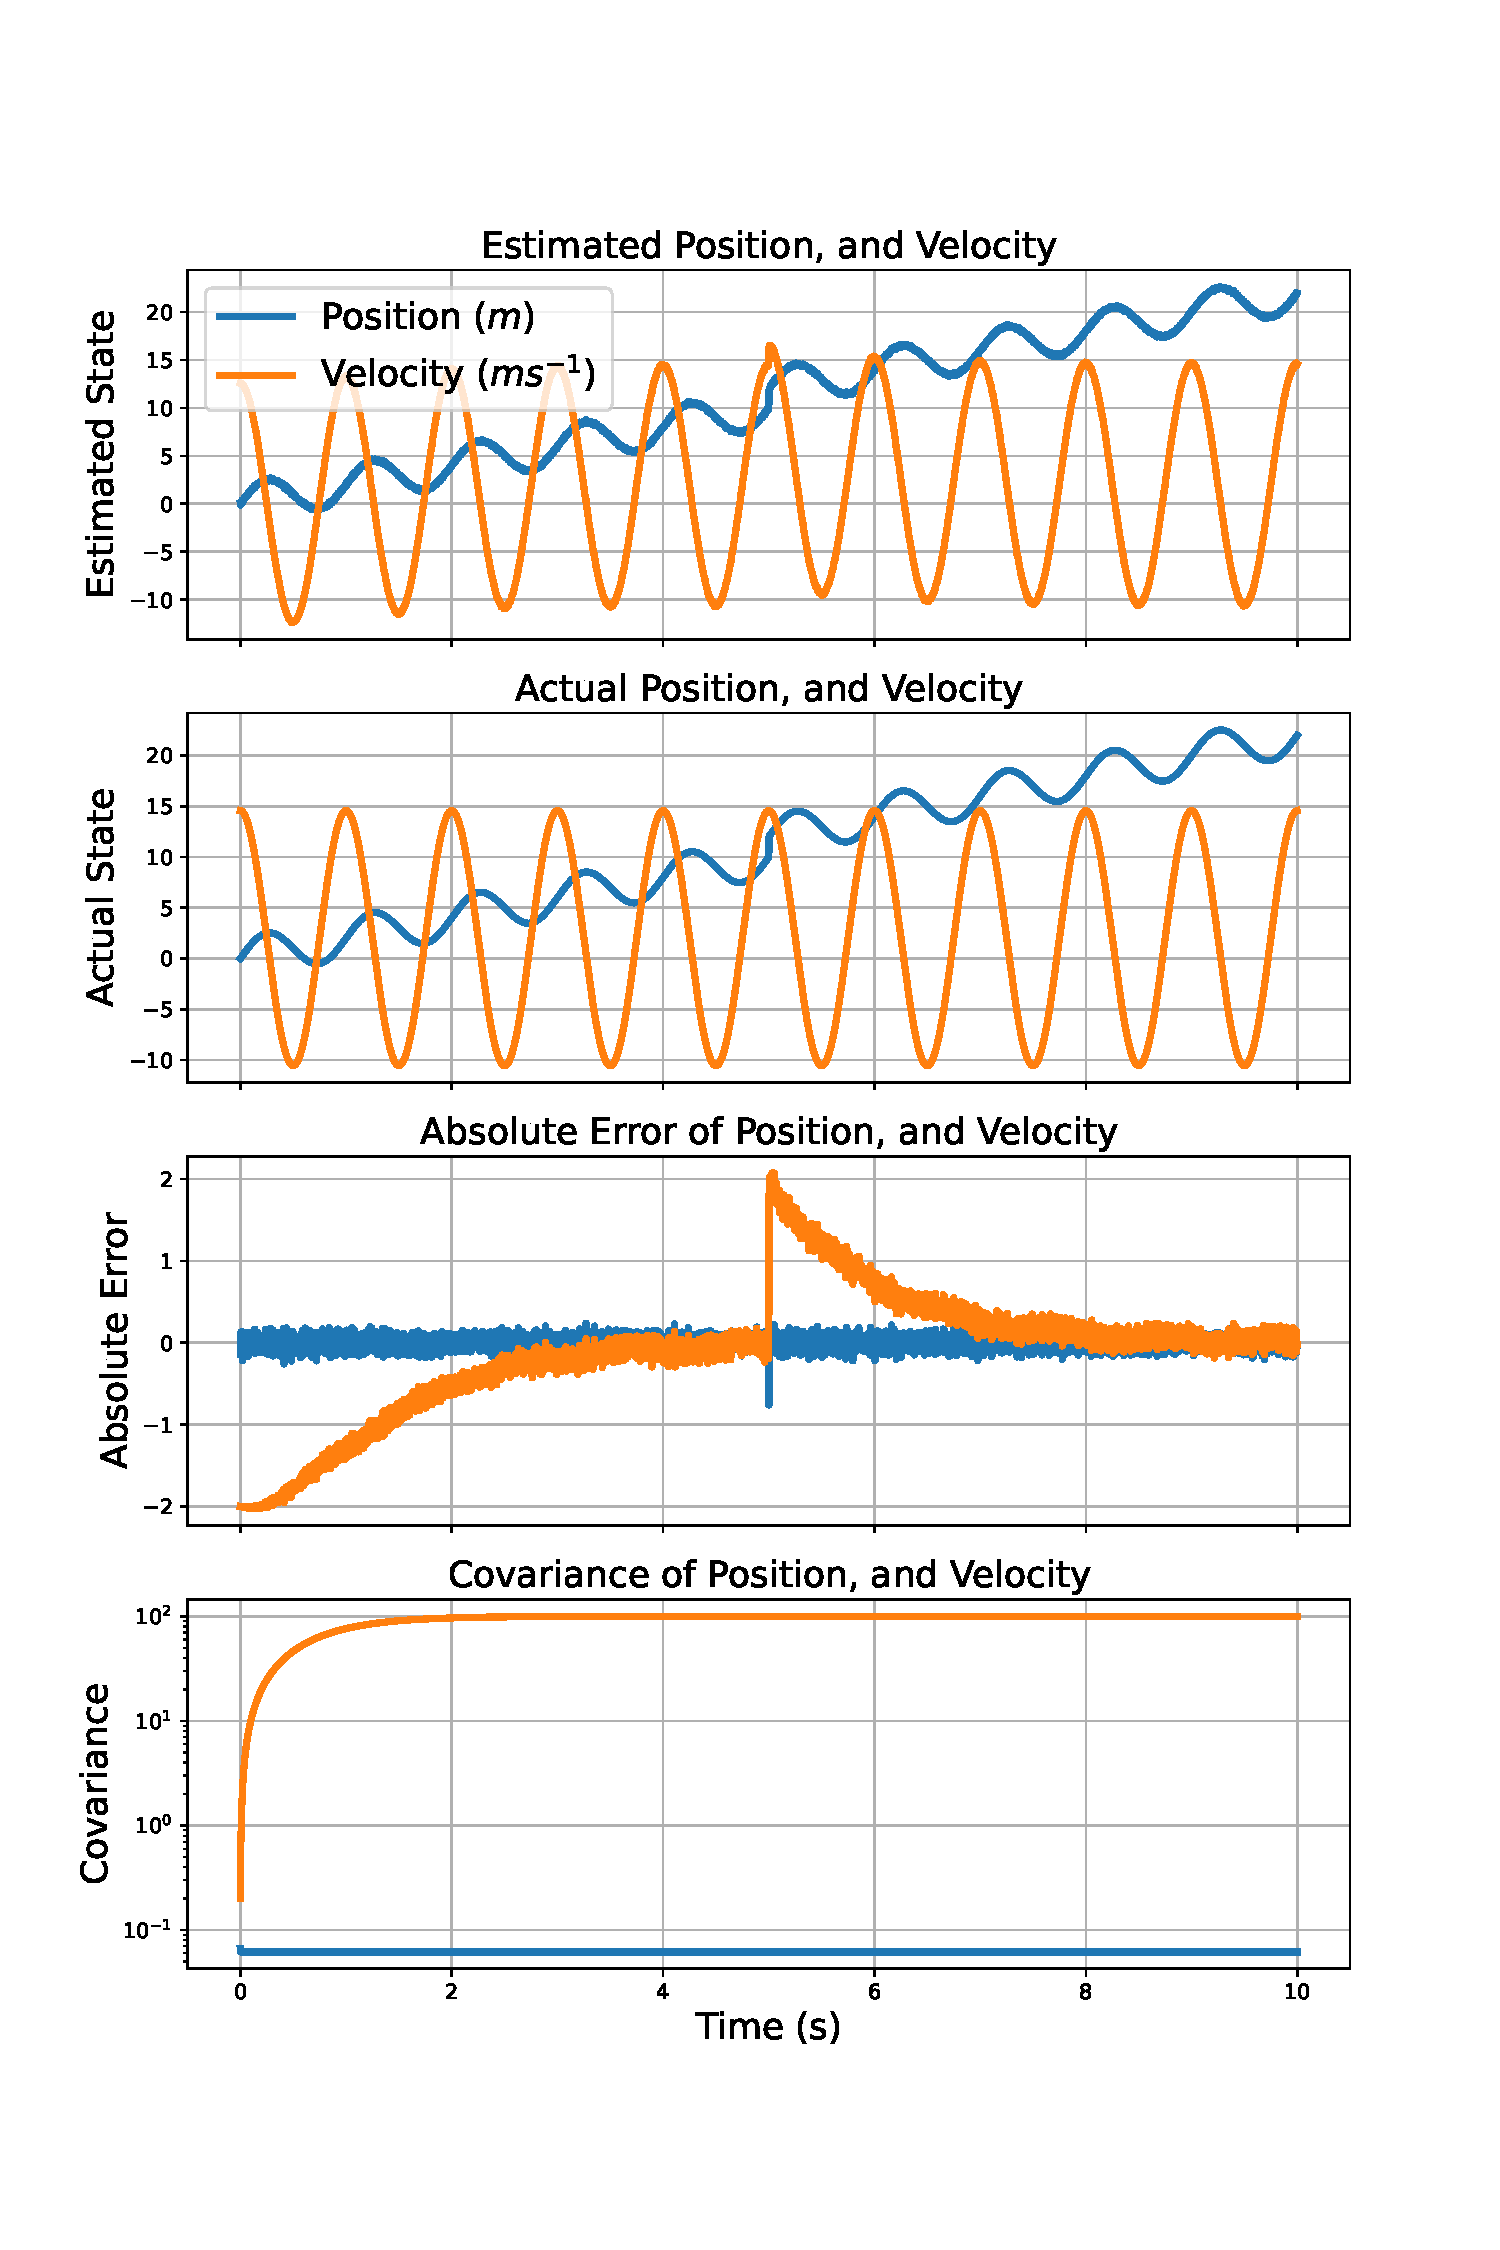
\includegraphics[width=\textwidth]{1d-position.pdf}
	
	\caption{A cart moving backwards and forwards, with a slight tendency to move in the positive direction. The cart is ``bumped'' at $t=5$, where we see the error of the velocity increase, until it settles down into a new equilibrium}
	\label{1d_position_fig}
\end{figure}

The next system was the same as before except the velocity was measured, and the position determined by integrating---i.e.\@ by adding the velocity multiplied by the time step to the position. In this scenario, the velocity is cyclical, with a slight increase over time. As we can see in figure \ref{1d_velocity_fig}, the model continues to perform well, with minimal error that appears to be bounded.

\begin{figure}[thp]
	\centering
	
	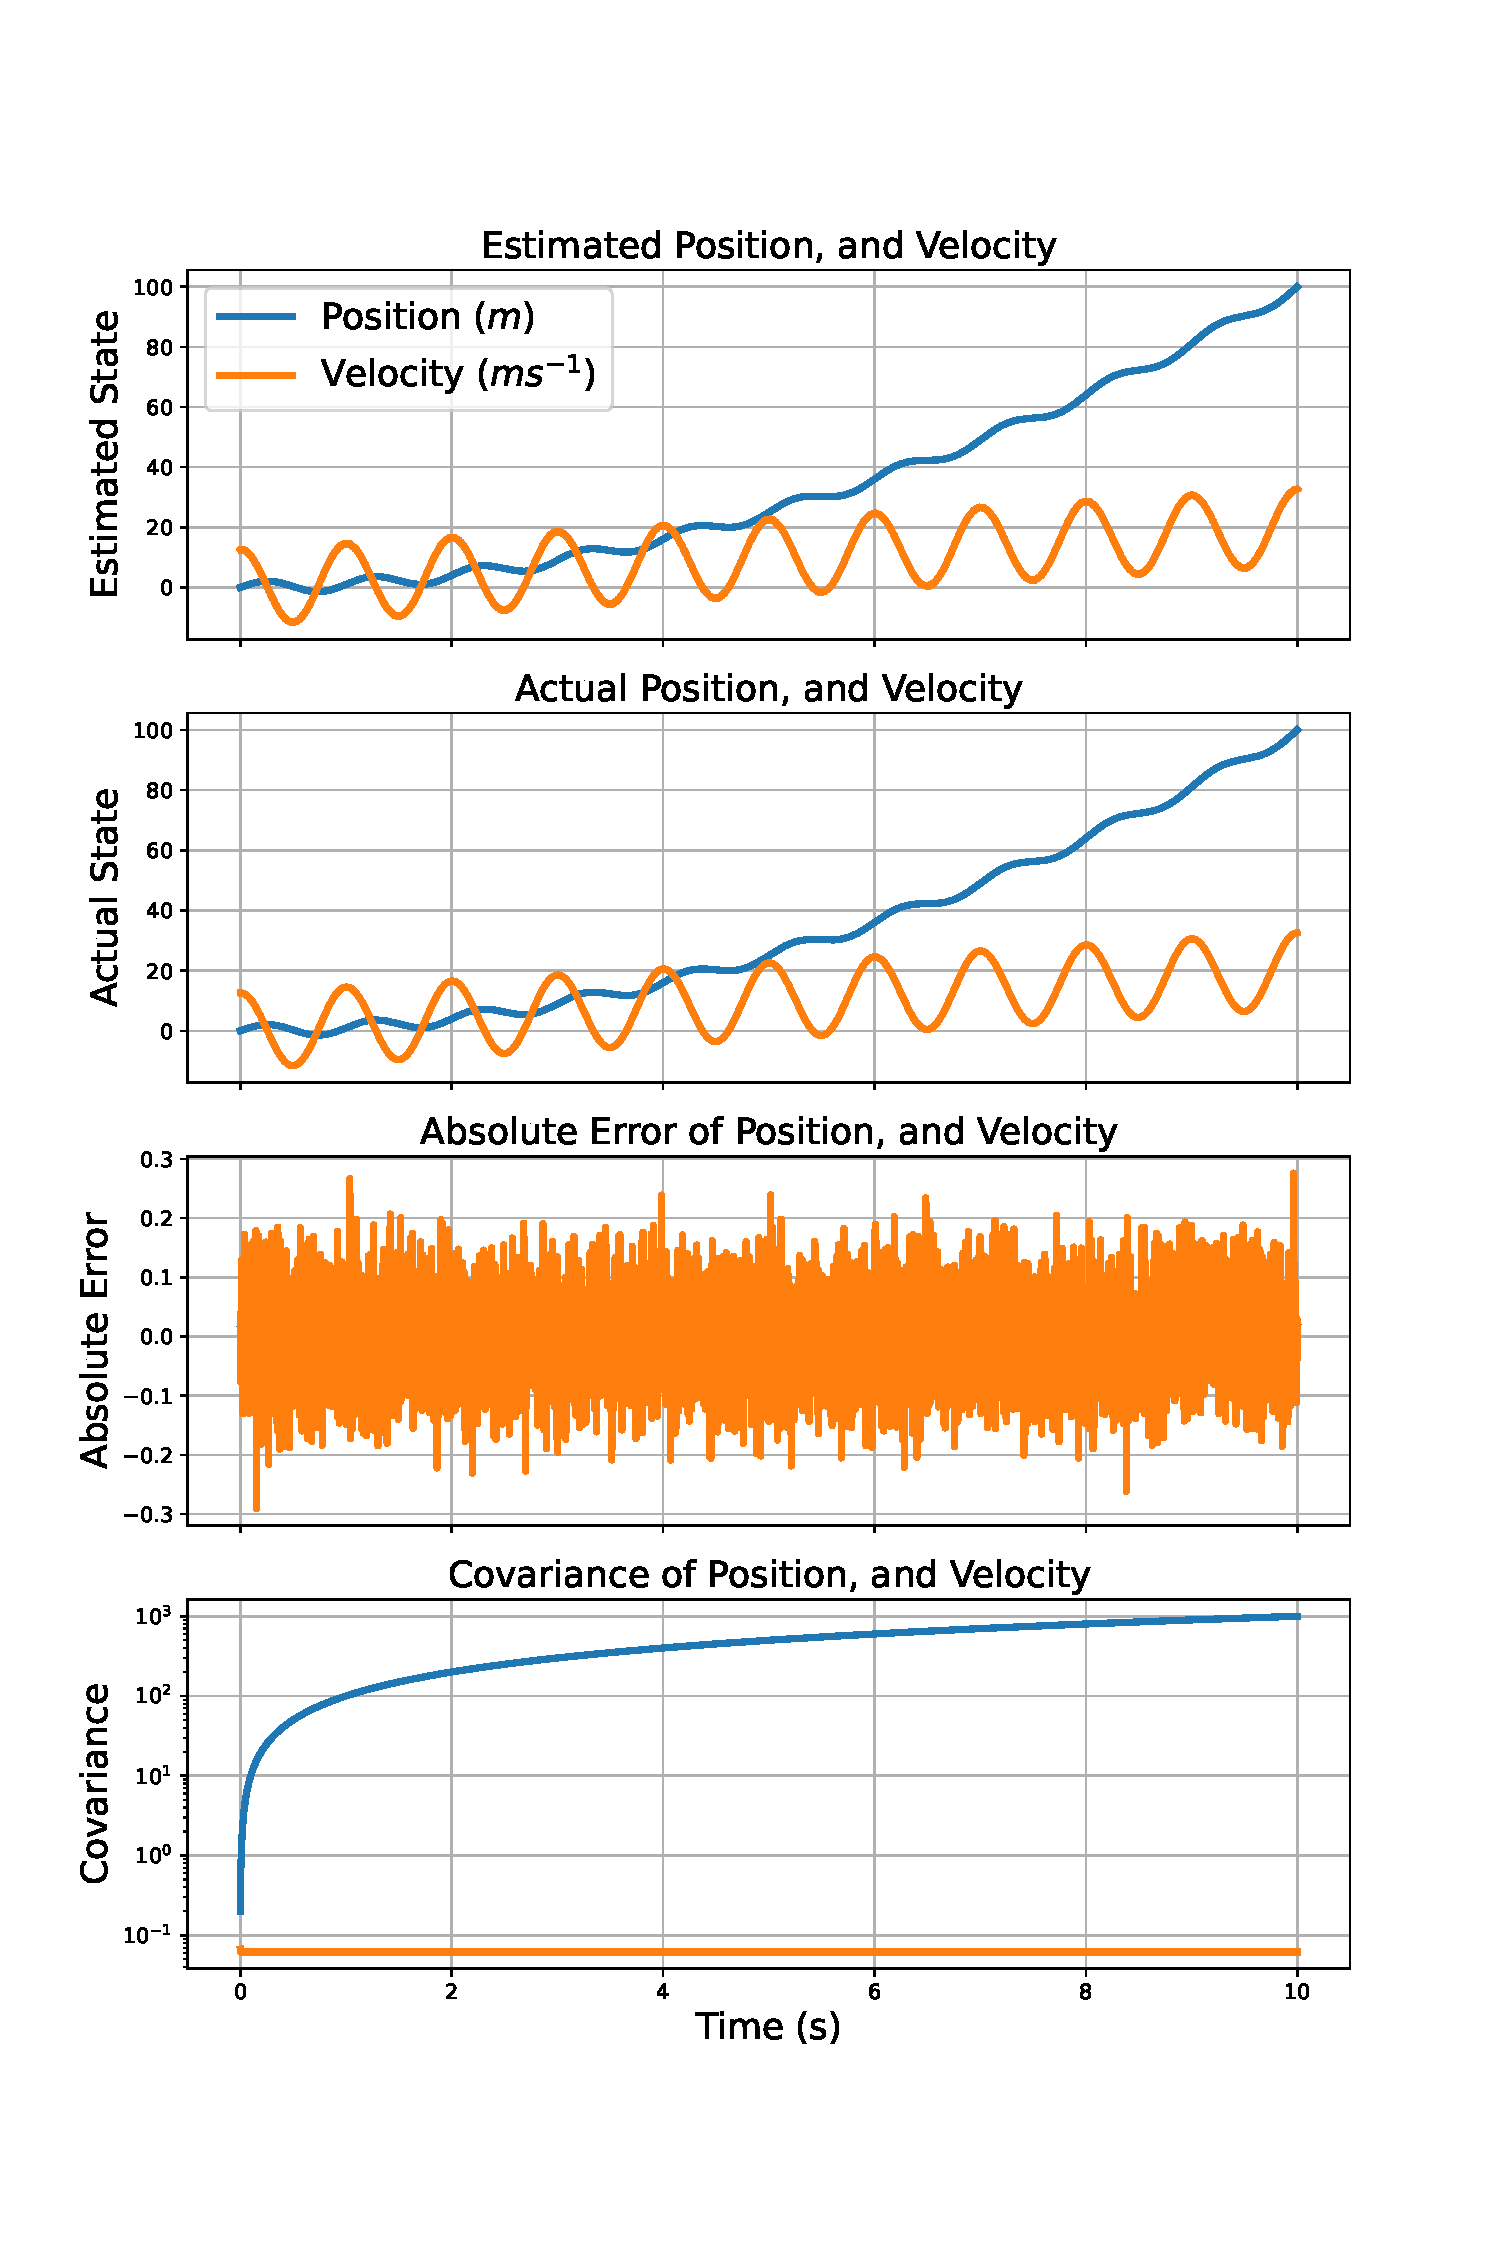
\includegraphics[width=\textwidth]{1d-velocity.pdf}
	
	\caption{Here we see the estimate of the state continue to be fairly accurate, even when faced with an unconstrained motion in the positive direction}
	\label{1d_velocity_fig}
\end{figure}

The final scenario is that of a three-dimensional body rocking backwards and forwards on all three axes. This also shows decent performance, which we can see in figure \ref{3d_orient_fig}. The error is low, and more importantly stays low (i.e.\@ doesn't run off to infinity).

\begin{figure}[thp]
	\centering
	
	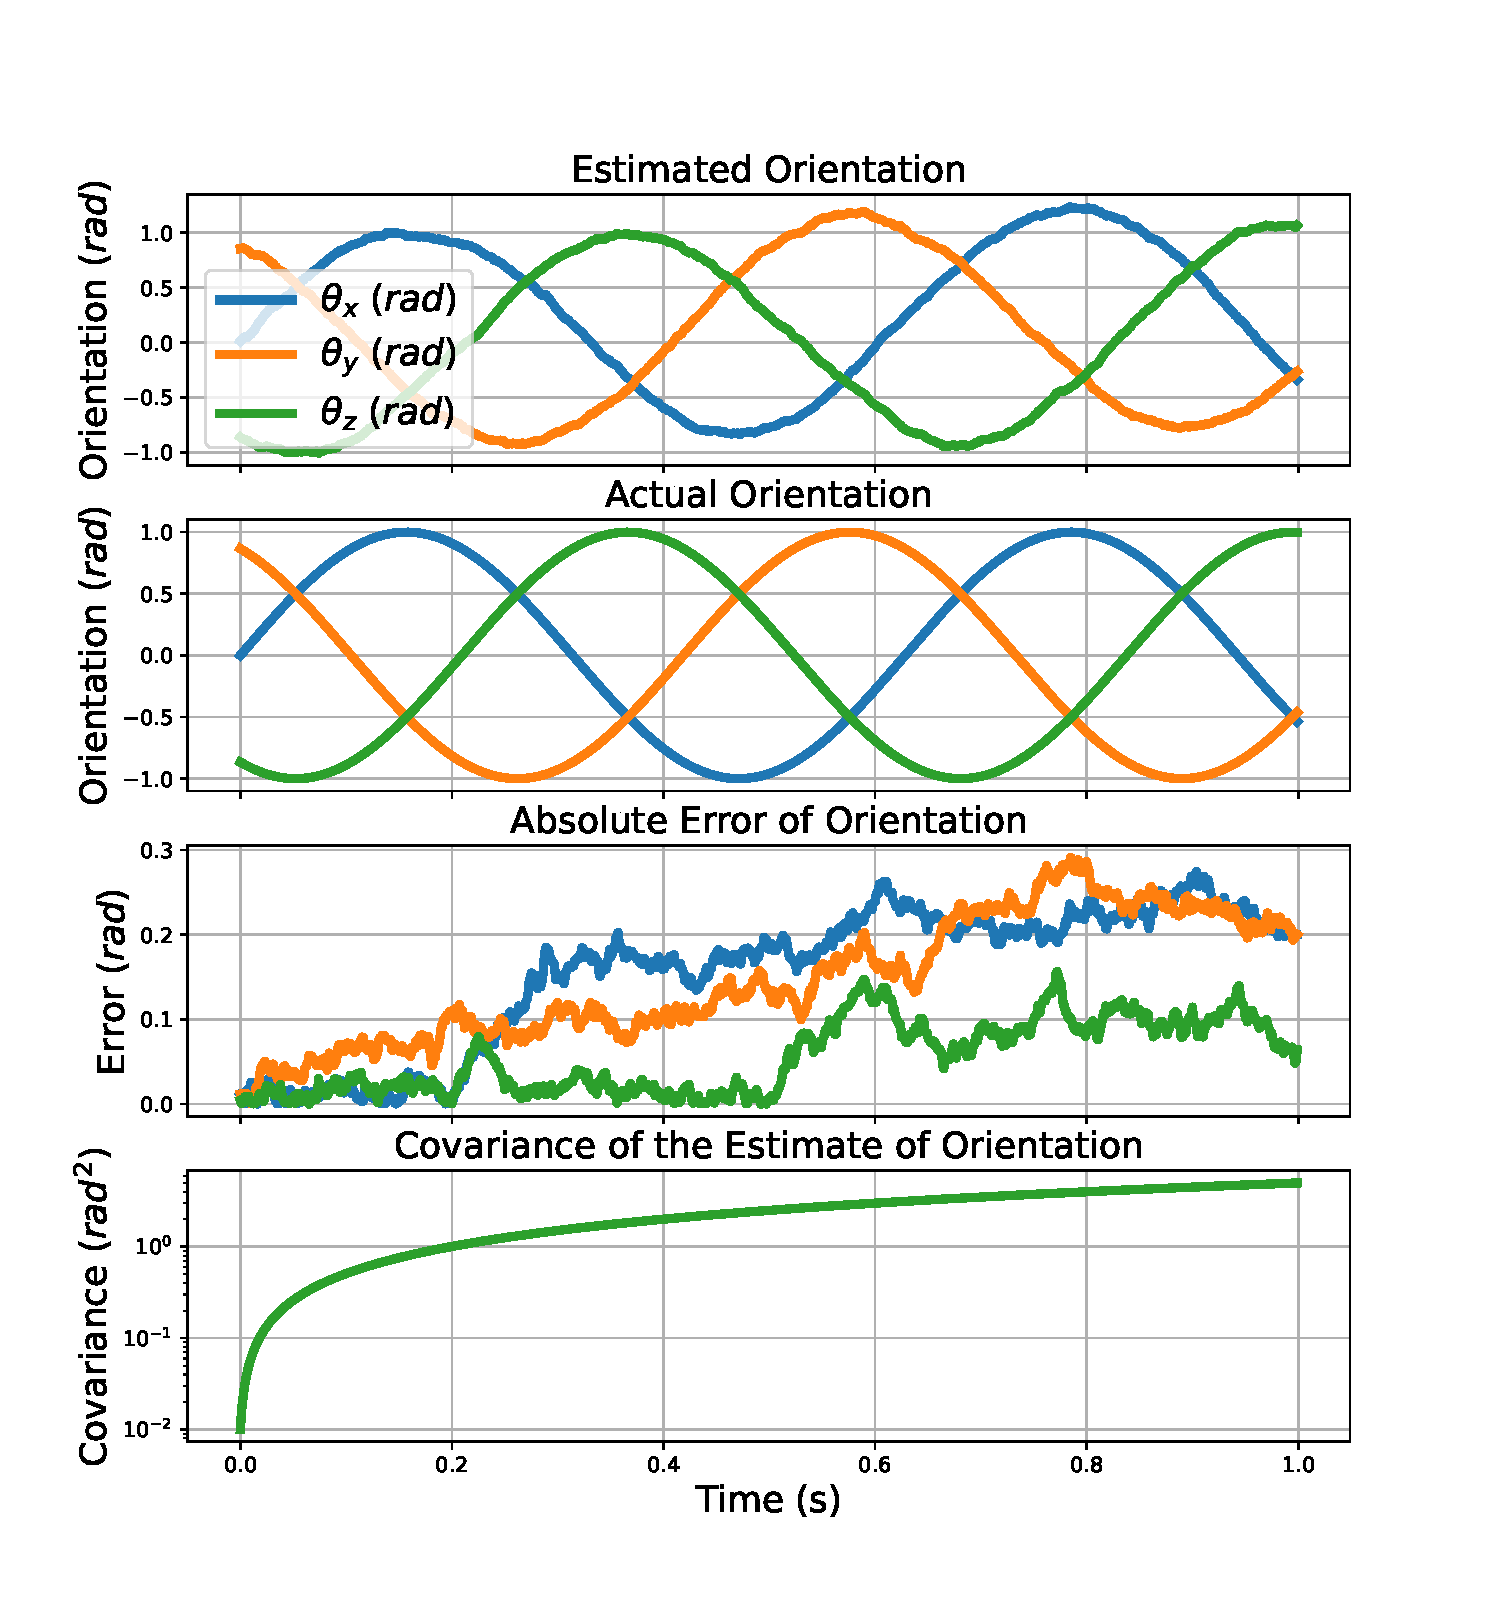
\includegraphics[width=\textwidth]{3d-orientation.pdf}
	
	\caption{A decent estimate of the orientation given noisy data. The covariance grows slowly.}
	\label{3d_orient_fig}
\end{figure}

From this we can also demonstrate how sensor and model noise affect the accuracy of the orientation estimate. For a discrete data set, the root-mean-square is defined as the square of the average of those values squared, i.e.

\begin{equation}
	x_{RMS} = \sqrt{{1 \over n}(x_1^2 + x_2^2 + \dots + x_n^2)}
\end{equation}

If we run multiple iterations of the three dimensional scenario, altering the amount of noise added the the measurements and system each time, we can calculate the RMS of the error values and plot that against that noise figure, as shown in figure \ref{3d_rms_fig}.

\begin{figure}[thp]
	\centering
	
	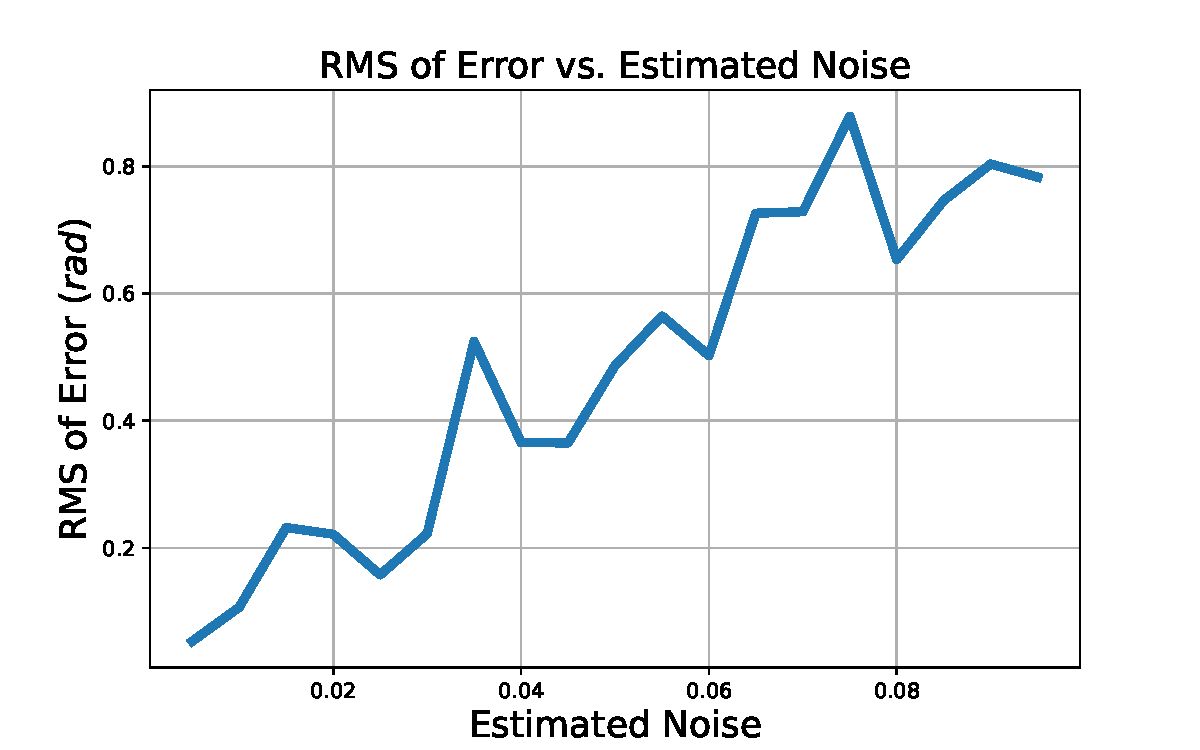
\includegraphics[width=\textwidth]{3d-rms.pdf}
	
	\caption{A plot showing the average error increasing as the amount of noise increases. The growth is approximately linear, with a slope of 9.23}
	
	\label{3d_rms_fig}
\end{figure}

Here we see linear growth (with some noise)---as we make the simulated sensors more noisy the quality of the output goes down. We can see the effect of this noise in figure \ref{3d_noise_fig}---where the noise is five times greater than in figure \ref{3d_orient_fig}.

\begin{figure}[thp]
	\centering
	
	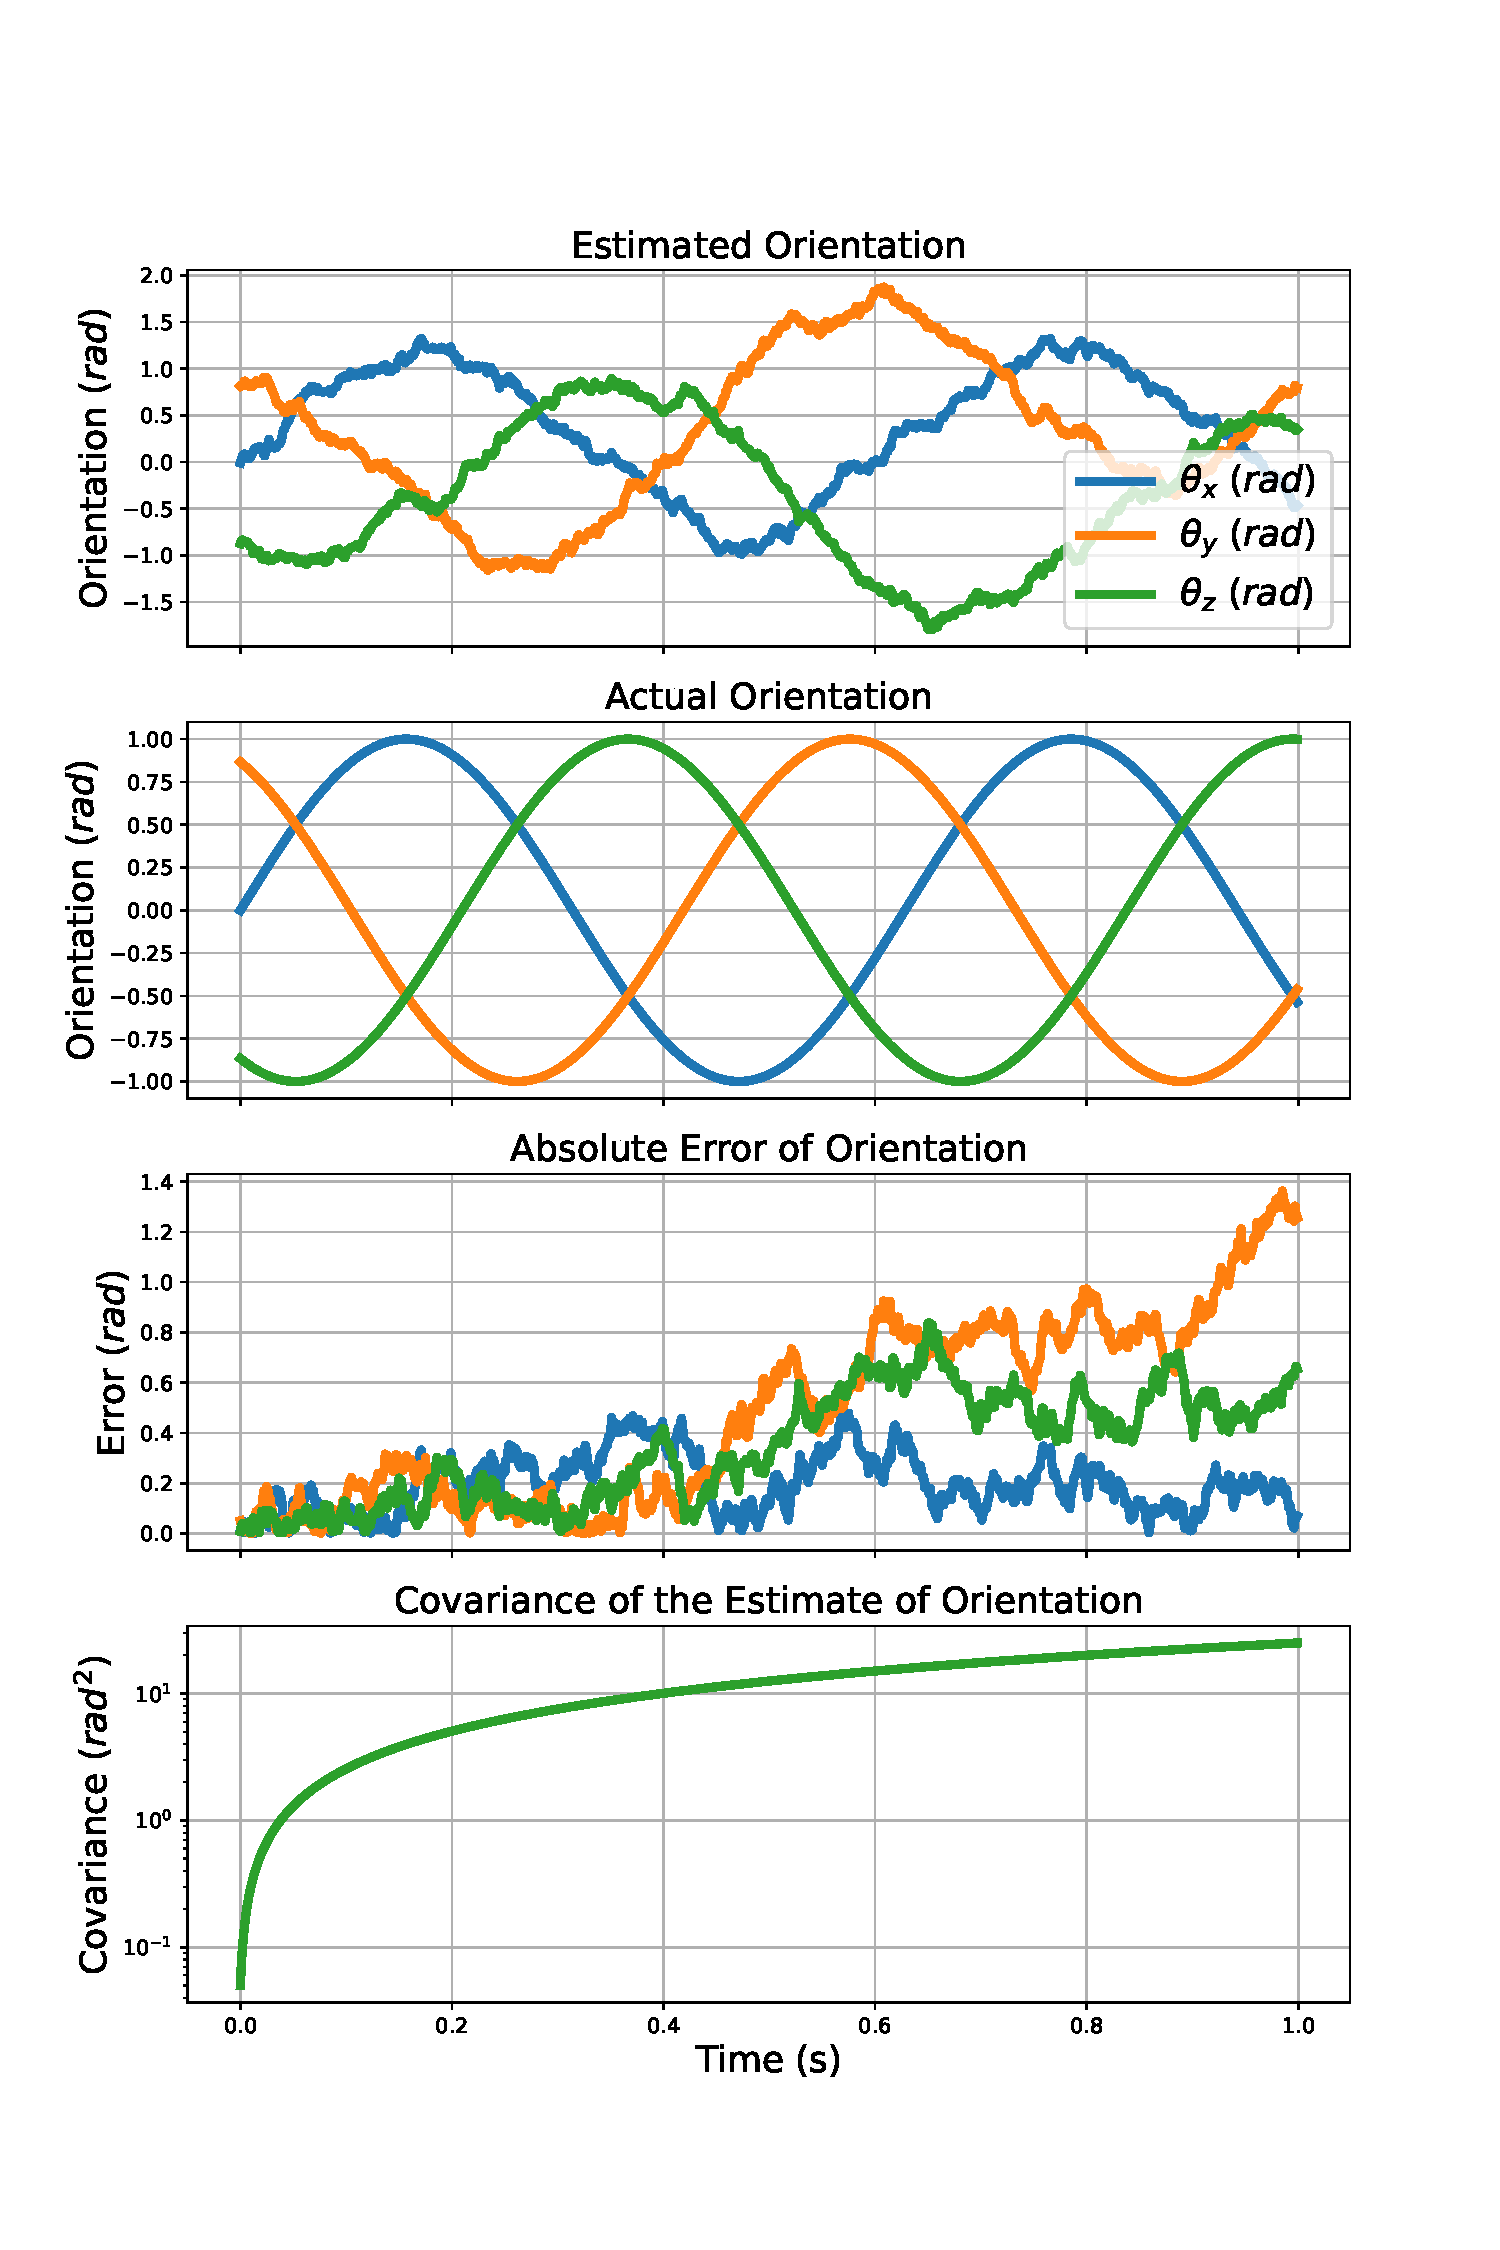
\includegraphics[width=\textwidth]{3d-orientation-noisy.pdf}
	
	\caption{The filter performing much worse---but the error is still bounded---and the shape of the periodic curves does approximately match reality}
	\label{3d_noise_fig}
\end{figure}

\subsection{Verilog Implementation}

As we have seen in \ref{recursion_space}, the amount of Verilog code required to perform a simple operation is quite vast. The $4\times4$ code I show could be written by hand fairly easily, however this would not be possible for the $12 \times 12$ matrix required for three dimensions each of orientation, acceleration, angular velocity, and the magnetic field vector---even a 9x9 version took up 40 slides in a beamer.

The solution is to automatically generate the Verilog code in software---this is the approach I used for the code in \ref{recursion_space}. This is not a trivial task but it is significantly easier to write a few hundred lines of Python than 20 KiB of Verilog.

So far, I have a reliable tool to generate the Verilog for calculating the determinant of arbitrarily sized matrices (with the maximum size specified when the Verilog is generated). I have also created a testbench module to confirm that it is, in fact, reliable.

\section{Future Work}

The remainder of the year will be dedicated to finishing the Verilog code / generation, and then evaluating its performance.

Certain specific tasks include:

\begin{itemize}
	\item Consider moving the orientation representations from angles to quaternions---this would take about one week, and would require re-writing how the mathematics works in both the Python and Verilog implementations.
	\item Adding matrix multiplication, inversion and transpose modules, and writing a Python ``compiler'' to compile a given mathematical equation to Verilog---this would take about two weeks, and would mostly require adapting the existing determinant code to the other operations, as well as developing the ``compiler'' to generate a ``glue'' module which would connect all the operations together.
	\item Reduce the amount of multipliers used, i.e.\@ by pipelining some of the common operations \cite{wang_2016}---this would take about two weeks, and would involve a rewrite of how multipliers are allocated to the matrix operation modules.
	\item Add the sensor interface Verilog code---this would take less than one week, and would involve creating a SPI or I2C module, which would be fairly straightforward.
	\item Verifying that it operates correctly, by comparing it to the Python implementation---this would take less than one week, and would mainly involve adding some method to log data from the FPGA to a computer, e.g.\@ via a UART module.
	\item Comparing the performance when preferring more precise sensor readings versus more frequent sensor readings---this would take about one week, and would be fairly straightforward, e.g.\@ changing clock frequencies and data bus widths.
\end{itemize}

\end{abstract}

\printbibliography

% Activate the appendix
% from now on sections are numerated with capital letters
\appendix

\renewcommand{\thesection}{Appendix \Alph{section}}

\section{Example of Recursion in Time}
\label{recursion_time}

\lstinputlisting[language=Python]{recursion-time.py}

\section{Example of Recursion in Space}
\label{recursion_space}

\lstinputlisting[language=Verilog]{recursion-space.v}

\section{Aims and Objectives}

\subsection*{Original}

\paragraph{Aims}

The aim of this project is to create an open source Verilog core for processing (in realtime) measurements from accelerometers, gyroscopes, and magnetometers to estimate the orientation and position of an object. This will be implemented on an FPGA to make an inertial navigation unit. This will then be compared to a software implementation in Python in order to validate performance and accuracy.

\paragraph{Objectives}

\begin{itemize}[noitemsep]
	\item Design a Kalman filter architecture (i.e.\@ what registers, the format of the input and output buses, etc.);
	\item Implement a Kalman filter in Python and produce input/output sample graphs using recorded data for some object (to give an illustration of what the Kalman filter is doing);
	\item Make a Verilog testbench (a module that runs some tests on another module, in this case the Kalman filter module);
	\item Create a Kalman filter Verilog module;
	\item Implement the Kalman filter module on an FPGA (possibly the Tang Nano);
	\item Make an inertial navigation unit from an FPGA and an SPI IMU module;
	\item Test and evaluate the accuracy of the inertial navigation unit;
	\item Explore the trade-off between arithmetic precision and accuracy versus power consumption;
	\item Validate its performance compared to the Python software implementation.
\end{itemize}

\subsection*{Revised}

\paragraph{Aims}

The aim of this project is to create an open source Verilog core for processing (in real time) measurements from accelerometers, gyroscopes, and magnetometers to estimate the orientation of an object. This will be implemented on an FPGA to make an inertial navigation unit. This will then be compared to a software implementation in Python in order to validate performance and accuracy.

\paragraph{Objectives}

\begin{itemize}[noitemsep]
	\item Implement a Kalman filter in Python and produce input/output sample graphs using recorded data for some object (to give an illustration of what the Kalman filter is doing);
	\item Make a Verilog testbench (a module that runs some tests on another module, in this case the Kalman filter module);
	\item Design a Kalman filter architecture (i.e.\@ what registers, the format of the input and output buses, etc.);
	\item Create a program to generate the Verilog modules for arbitrarily sized matrices
	\item Implement the Kalman filter design on an FPGA (possibly the Tang Nano, but likely something larger);
	\item Make an inertial navigation unit from an FPGA and an SPI IMU module;
	\item Test and evaluate the accuracy of the inertial navigation unit;
	\item Explore the trade-off between arithmetic precision and accuracy versus power consumption;
	\item Validate its performance compared to the Python software implementation.
\end{itemize}

\end{document}